\chapter{Introduction}

This User Guide provides a guideline for the configuration and integration of the ETAS developed RTA-SUM SSFM. RTA-SUM SSFM module has been developed towards the Software Defined Veichle requirements, specifically, the SDV-8002 specifications and related specifications listed in Section \ref{sec:GBReferences}.

\ifnum \DocumentGroup=1
{
General guidelines on the common steps and workflow for RTA-SUM integration can be found in RTA-SUM Getting Started Guide.
}
\else
{
%Nothing
}\fi

\section{Definitions and Abbreviations}
\input{generated/tables/definitions.tex}

\section{Module Overview}
The RTA-SUM SSFM, Signal Status and Fault Monitor, is a software composition located in the Application Layer of the standardized architecture of AUTOSAR.

SSFM interprets the various "status" of the data value which are associated with received serial data signals and provides a consistent interface to functional software. 
\textbf{SUM\_SSFM} functionality is composed of two logic units:
\begin{itemize}
	\item \textbf{Signal Status Monitoring logic}: This logic is handling the monitoring of the serial data signal status to detect various types of faults such as loss of communication, safety protection errors and security verification errors. This logic unit is referred to as Signal Status Monitor (SSM) throughout the rest of this specification. SSM is not a separate Software component but a logic unit inside the SUM\_SSFM software component.
	\item \textbf{Fault Reporting logic}: This logic is mainly handling the maturation and filtering of the faults detected by the SSM logic and reporting the faults to the AUTOSAR Dem module. It is also responsible for other error handling functionalities such as BSW production error events aggregation and Precondition Check for Control DTC settings for instance. This logic is referred to as Error Handler (ERRH) throughout the rest of this specification. ERRH is not a separate Software component but a logic unit inside the SUM\_SSFM software component.
\end{itemize}

\textbf{SSM} implements the following functionalities:
\begin{itemize}
	\item Consolidate ECU internal conditions to determine signal status for use by functional software.
	\item Use Security verification status notification from AUTOSAR SecOC module via a Sender/Receiver Interface to notify applications on the security authentication status of the authenticated PDUs.
	\item Use initialization and startup conditions to define signal status before serial communication is active/reception of signals.
	\item Integrate relevant status monitor signals of the received signal to calculate status information
	\item Aggregate signal supervision status from a source to determine Node Loss conditions.
	\item Disable the transmission of PDUs for variant handling.
	\item Map the AUTOSAR E2E transformer checking status during the checking of safety signals received within a protected SerialData and provide a consistent interface to functional software.
\end{itemize}

\textbf{ERRH} implements the following functionalities:
\begin{itemize}
	\item Aggregation of BSW production error events from Dem
	\item Aggregation of SUM error events from each SUM
	\item Aggregation of deadline monitoring events from SSM for signals which are relevant to setting of node loss U-code DTC(s)
	\item Aggregation of DTC list from Dem
	\item Precondition Check for Control DTC Setting request from DCM based on Channel and Tester information.
\end{itemize}

\begin{center}
	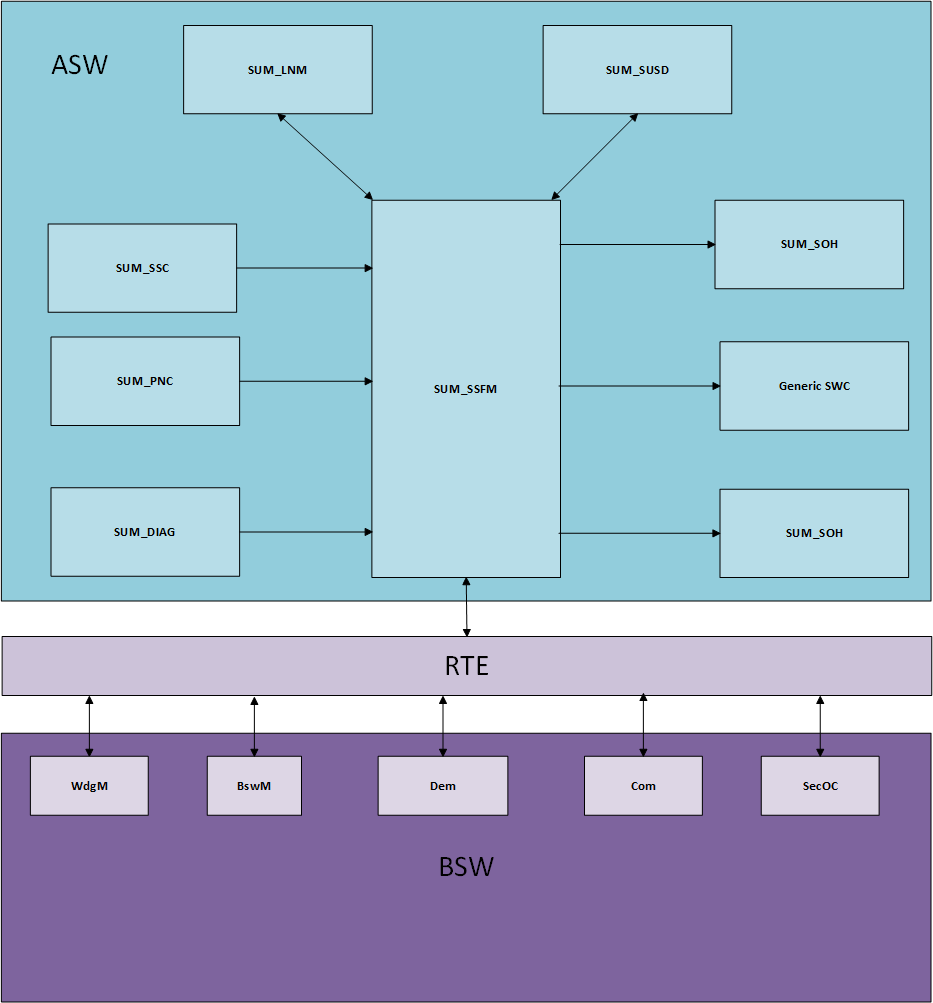
\includegraphics[scale=0.7]{images/SSFM_System_Block_View.png}
\end{center}

\section{References}
\label{sec:GBReferences}
\input{generated/tables/references.tex}
